\documentclass[a4paper,12pt]{article} 

%%% Работа с русским языком
\usepackage{cmap}					% поиск в PDF
\usepackage{mathtext} 				% русские буквы в фомулах
\usepackage[T2A]{fontenc}			% кодировка
\usepackage[utf8]{inputenc}			% кодировка исходного текста
\usepackage[english,russian]{babel}	% локализация и переносы

%%% Дополнительная работа с математикой
\usepackage{amsmath,amsfonts,amssymb,amsthm,mathtools, gensymb} % AMS
\usepackage{icomma} % "Умная" запятая: $0,2$    ф--- число, $0, 2$ --- перечисление

%%Таблица
\usepackage[table,xcdraw]{xcolor}
\usepackage{caption}
\usepackage{floatrow}
\floatsetup[table]{capposition=top}
\floatsetup[wrapfigure]{capposition=bottom}
\usepackage{multirow}

%Отступы и поля 
\textwidth=18cm
\oddsidemargin=-1cm
\topmargin=-2cm
\textheight=25cm


%% Номера формул
\mathtoolsset{showonlyrefs=true} % Показывать номера только у тех формул, на которые есть \eqref{} в тексте.

%% Шрифты
\usepackage{euscript}	 % Шрифт Евклид
\usepackage{mathrsfs} % Красивый матшрифт

%% Свои команды
\DeclareMathOperator{\sgn}{\mathop{sgn}}

%% Перенос знаков в формулах (по Львовскому)
\newcommand*{\hm}[1]{#1\nobreak\discretionary{}
{\hbox{$\mathsurround=0pt #1$}}{}}

%% Стиль страницы
\usepackage{fancyhdr}

%% Для рисунков
\usepackage{graphicx}
\usepackage[export]{adjustbox}
\usepackage{float}
\usepackage{ragged2e}
\usepackage{wrapfig}

\pagestyle{fancy}
\begin{document}
\begin{titlepage}
\begin{center}
%\vspace*{1cm}
\large{\small ФЕДЕРАЛЬНОЕ ГОСУДАРСТВЕННОЕ АВТОНОМНОЕ ОБРАЗОВАТЕЛЬНОЕ\\ УЧРЕЖДЕНИЕ ВЫСШЕГО ОБРАЗОВАНИЯ \\ МОСКОВСКИЙ ФИЗИКО-ТЕХНИЧЕСКИЙ ИНСТИТУТ\\ (НАЦИОНАЛЬНЫЙ ИССЛЕДОВАТЕЛЬСКИЙ УНИВЕРСИТЕТ)\\ ФАКУЛЬТЕТ АЭРОКОСМИЧЕСКИХ ТЕХНОЛОГИЙ}
\vfill
\line(1,0){490}\\[1mm]
\huge{Лабораторная работа 4.7.1}\\
\huge\textbf{Двойное лучепреломление}\\
\line(1,0){490}\\[1mm]
\vfill
\begin{flushright}
\normalsize{Рогозин Владимир}\\
\normalsize{\textbf{Группа Б03-106}}\\
\end{flushright}
\end{center}
\end{titlepage}
\fancyhead[L] {Работа 4.7.1}

\textbf{Цель работы}: 
Изучение зависимости показателя преломления необыкновенной волны от направления в двоякопреломляющем кристалле; определение главных показателей преломления $n_o$ -- обыкновенной и $n_e$ -- необыкновенной волны в кристалле; наблюдение эффекта полного внутреннего отражения.

\textbf{Оборудование}:
Гелий-неоновый лазер, вращающийся столик с неподвижным лимбом, призма из исландского шпата, поляроид.

\textbf{Теоретические сведения}:
При падении световой волны на границу \textit{изотропной} среды в этой среде от границы распространяется одна волна. Если среда \textit{анизотропна}, то в ней в общем случае возникают две волны, распространяющиеся от границы в разных направлениях и с разными скоростями. Это явление и исследуется в нашей работе.

\textbf{Плоские волны в кристаллах.}
Фундаментальные уравнения Максвелла справедливы без всяких изменений и в кристаллических средах. В отсутствие электрических зарядов и токов они имеют вид
\begin{equation}\label{eq: Maxwell equations}
    \operatorname{rot\mathbf{H}} = \frac{1}{c} \frac{\partial\mathbf{D}}{\partial t}, \quad \operatorname{rot\mathbf{E}} = -\frac{1}{c} \frac{\partial\mathbf{B}}{\partial t}.
\end{equation}\
Если среды \textit{прозрачны} и \textit{однородны}, то в них могут распространяться плоские монохроматические волны. Запишем такую волну в комплексном виде:
\begin{equation}\label{eq: Monochrom. waves}
    \mathbf{E} = \mathbf{E_0} e^{i(\omega t - \mathbf{k}\mathbf{r})}, \quad
    \mathbf{B} = \mathbf{H} = \mathbf{H_0} e^{i(\omega t - \mathbf{k}\mathbf{r})}, \quad
    \mathbf{D} = \mathbf{D_0} e^{i(\omega t - \mathbf{k}\mathbf{r})}.
\end{equation}
Здесь $\omega$ -- круговая частота, $\mathbf{k}$ -- волновой вектор, а амплитуды $\mathbf{E_0}$, $\mathbf{H_0}$, $\mathbf{D_0}$ постоянны. Вектор $\mathbf{B}$ совпадает с $\mathbf{H}$, так как $\mu = 1$. Из соотношений \eqref{eq: Maxwell equations} и \eqref{eq: Monochrom. waves} получаем:
\begin{equation}\label{eq: D and H via N}
    \mathbf{D} = -\frac{c}{v} \Big[\mathbf{N} \times \mathbf{H}\Big], \quad
    \mathbf{B} = \frac{c}{v} \Big[\mathbf{N} \times \mathbf{E}\Big], \quad
    \mathbf{N} = \frac{v}{\omega}\mathbf{k}
\end{equation}
Из полученных уравнений видно, что векторы $\mathbf{D}, \mathbf{H}, \mathbf{N}$ взаимно перпендикулярны, а значит плоские волны в кристалле поперечны в отношении векторов $\mathbf{D}$ и $\mathbf{H}$. Однако в общем случае они не поперечны в отношении вектора $\mathbf{E}$. 

\begin{wrapfigure}[19]{l}{0.4\textwidth}\label{fig: Vectors' location}
    \begin{center}
    \vspace{-20pt}
        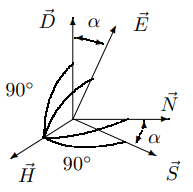
\includegraphics[width = 0.9\textwidth]{Vectors' location.png}
    \end{center}
    \caption{Расположение векторов $\mathbf{D}$, $\mathbf{E}$, $\mathbf{N}$, $\mathbf{S}$ в анизотропной среде}
\end{wrapfigure}
В изотропной среде связь между вектором напряжённости электрического поля $\mathbf{E}$ и вектором индукции $\mathbf{D}$ даётся материальным уравнением $\mathbf{D} = \varepsilon\mathbf{E}$, где $\varepsilon$ -- постоянная, не зависящая от направления величина, называемая \textit{диэлектрической проницаемостью}. Для характеристики оптических свойств анизотропной среды требуется девять величин $\varepsilon_{ij}$ , образующих \textit{тензор диэлектрической проницаемости}:
\begin{equation}\label{eq: Tenzor eps}
    D_i = \sum_j \varepsilon_{ij}E_j 
\end{equation}
Благодаря тензорной связи между $\mathbf{D}$ и $\mathbf{E}$ направления этих векторов в кристаллах, вообще говоря, не совпадают. Плоскость $\big(\mathbf{E}, \mathbf{H}\big)$ обладает тем свойством, что перпендикуляр к ней определяет направление вектора Пойнтинга, т.е. направление распространения световых
лучей. Четыре вектора $\mathbf{D}$ , $\mathbf{E}$ , $\mathbf{N}$ , $\mathbf{S}$ лежат в одной плоскости, перпендикулярной вектору $\mathbf{H}$. Взаимное расположение этих векторов показано на рис. 1. 

\textbf{Оптически одноосные кристаллы.} 
Всю совокупность возможных значений тензора диэлектрической проницаемости можно представить при помощи трёхосного эллипсоида. Значение диэлектрической проницаемости для любого направления выражается длиной радиуса-вектора эллипсоида, проведенного по этому направлению. Три значения диэлектричеcкой проницаемости $\varepsilon_x$, $\varepsilon_y$, $\varepsilon_z$, соответствующие осям эллипсоида, называются \textit{главными значениями диэлектрической проницаемости} и соответственно $\sqrt{\varepsilon_x}$, $\sqrt{\varepsilon_y}$, $\sqrt{\varepsilon_z}$ -- \textit{главными показателями преломления}.

В системе координат, оси которой совпадают с главными осями эллипсоида, тензор диэлектрической проницаемости приводится к диагональному виду. В оптически одноосном кристалле, каковым является исландский шпат, эллипсоид диэлектрической проницаемости представляет собой эллипсоид вращения. В нем оптическая ось -- определённое направление в кристалле, вдоль которого лучи с ортогональной поляризацией распространяются с одной скоростью, как в обычной изотропной среде, а $\varepsilon$ имеет экстремальное значение, совпадает с осью вращения эллипсоида диэлектрических проницаемостей. Для главных значений диэлектрических проницаемостей приняты обозначения: $\varepsilon_z = \varepsilon_{\|}$ и $\varepsilon_x = \varepsilon_x = \varepsilon_{\perp}$.

\begin{wrapfigure}[20]{l}{0.4\textwidth}\label{fig: Vectors' location crystal}
    \begin{center}
    \vspace{-20pt}
        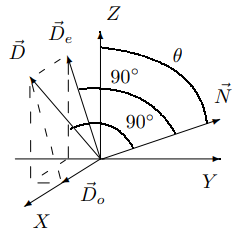
\includegraphics[width = 0.9\textwidth]{Vectors' location crystal.png}
    \end{center}
    \caption{Расположение векторов $\mathbf{D}$ и $\mathbf{N}$ в анизотропной среде}
\end{wrapfigure}
Волну, распространяющуюся в одноосном кристалле, можно разделить на две линейно
поляризованные волны: \textit{обыкновенную}, вектор электрической индукции $\mathbf{D}_o$ которой перпендикулярен главному сечению, и \textit{необыкновенную}, с вектором электрической индукции
$\mathbf{D}_e$, лежащим в главном сечении. \textit{Главным сечением кристалла} называется плоскость, в которой лежит оптическая ось кристалла и нормаль к фронту волны.

Рассмотрим вначале обыкновенную волну, в которой вектор $\mathbf{D_o}$ перпендикулярен главному сечению. Тогда $\mathbf{D_{oz}} = 0$, а значит $\mathbf{E_{oz}} = 0$. Принимая во внимание $\varepsilon_y = \varepsilon_x = 
\varepsilon_{\perp}$, получаем,что для обыкновенной волны материальное уравнение имеет такой же вид, как и в изотропной среде
\[\mathbf{D_{o}} = \varepsilon_{\perp} \mathbf{E_{o}},\]
откуда 
\[n_o = \frac{c}{v_0} = \sqrt{\varepsilon_{\perp}}.\]
Таким образом, скорость распространения обыкновенной волны
и ее показатель преломления не зависят от направления распространения.

Для того чтобы найти скорость распространения v и показатель преломления необыкновенной волны $n = c/v$, достаточно найти связь между вектором электрической индукции этой волны
$\mathbf{D_e}$ и проекцией на него вектора электрического поля волны $E_{eD}$.
\begin{equation}\label{eq: E_eD}
    E_{eD} = \frac{\mathbf{E_e}\mathbf{D_e}}{D_e} = \frac{D^2_{e\|} / \varepsilon_\| + D^2_{e\perp} / \varepsilon_\perp}{D_e} = D_e\bigg( \frac{\sin^2\theta}{\varepsilon_\|} + \frac{\cos^2\theta}{\varepsilon_\perp}\bigg) = \frac{D_e}{\varepsilon}, 
\end{equation}
где 
\[\sin\theta = \frac{D_{e\|}}{D_e}, \quad \cos\theta = \frac{D_{e\perp}}{D_{e}}.\]

Таким образом, $\varepsilon$ и соответственно скорость распространения и показатель преломления необыкновенной волны зависят от угла между оптической осью кристалла и направлением распространения волны.
\begin{equation}\label{eq: n}
    \frac{1}{[n(\theta)]^2} = \frac{\sin^2\theta}{n^2_e} + \frac{\cos^2\theta}{n^2_o}
\end{equation}

При $n_o - n_e \ll n_o$ и $n_e$ выражение \eqref{eq: n} можно упростить:
\[n(\theta) \approx n_e + (n_o - n_e)\cos^2\theta.\]

\textbf{Двойное лучепреломление в призме из исландского шпата.} В исследуемой призме ось кристалла лежит в плоскости, параллельной верхней грани призмы, причем она параллельна входной грани призмы (длинному катету). При этом в обыкновенной волне вектор $\mathbf{D_o}$ перпендикулярен верхней грани призмы, а в необыкновенной волне вектор $\mathbf{D_e}$ параллелен верхней грани.
\begin{figure}[H]\label{fig: Prism}
    \centering
    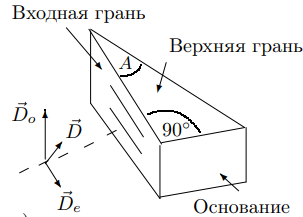
\includegraphics[width = 0.6\textwidth]{Prism.png}
    \caption{Исследуемая призма из исландского шпата. Штриховкой указано направление оптической оси кристалла.}
\end{figure}

\begin{wrapfigure}[19]{l}{0.4\textwidth}\label{fig: Rays in prism}
    \begin{center}
    \vspace{-20pt}
        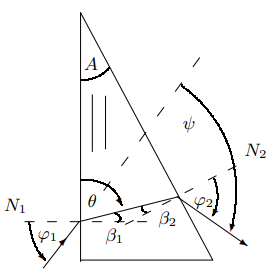
\includegraphics[width = 0.9\textwidth]{Rays in prism.png}
    \end{center}
    \caption{Ход лучей в призме}
\end{wrapfigure}
Волну, падающую на входную грань призмы, можно представить в виде суммы двух ортогональных линейно поляризованных волн. Преломление этих двух волн на грани призмы можно рассматривать независимо.

Значение показателя преломления и угол, под которым преломилась волна в призме, можно найти, измерив угол падения на входную грань призмы $\varphi_1$ и угол $\varphi_2$ на выходе призмы (рис. 4). Запишем закон Снеллиуса для одной из волн применительно к первой
и второй граням призмы:
\[\sin\varphi_1 = n \sin\beta_1;\]
\[\sin\varphi_2 = n\sin\beta_2 = n\sin(A - \beta_1).\]
Учитывая, что угол преломления $\beta_1$ связан с углом $\theta$ между осью кристалла
и волновой нормалью $\mathbf{N}$ соотношением $\theta + \beta_1 = \pi / 2$, находим $n$ и $\theta$:
\begin{equation}\label{eq: n in prism}
    n = \frac{1}{\sin A}\sqrt{\sin^2\varphi_1 + \sin^2\varphi_2 + 2\sin\varphi_1\sin\varphi_2\cos A};
\end{equation}
\[\cos\theta = \frac{\sin\varphi_1}{n}.\]

Показатель преломления призмы из изотропного материала удобно находить по углу наименьшего отклонения луча от первоначального направления. Угол отклонения луча призмой ($\psi$ на рис. 4) минимален для симметричного хода лучей, т.е. когда $\varphi_1 = \varphi_2$. Тогда показатель преломления можно рассчитать по формуле
\begin{equation}\label{eq: n via min psi}
    n = \frac{\sin(\frac{\psi_m + A}{2})}{\sin(\frac{A}{2})},
\end{equation}
где $\psi_m$ -- угол наименьшего отклонения.

\textbf{Экспериментальная установка}:
Схема экспериментальной установки изображена на рис. 5. Источником излучения служит Не-Nе лазер ($\lambda$ = 0,63 мкм)
\begin{figure}[H]\label{fig: Exp setup}
    \centering
    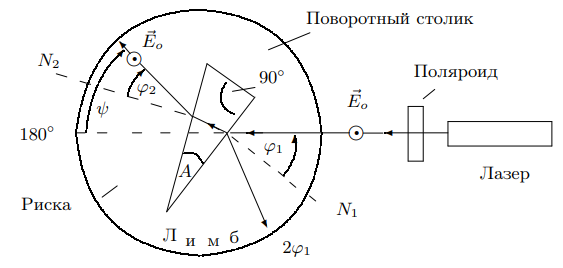
\includegraphics[width = 0.6\textwidth]{Exp setup.png}
    \caption{Исследуемая призма из исландского шпата. Штриховкой указано направление оптической оси кристалла.}
\end{figure}
Преломляющий угол $A$ призмы (рис. 4) можно рассчитать, если известны угловые
координаты нормалей $N_1$ и $N_2$ к преломляющим (рабочим) граням призмы, прилежащим преломляющему углу.

Угол падения $\varphi_1$ определяется по положению луча, отражённого от передней (входной) грани призмы (рис. 5). Из рис. 4 можно получить связь углов $\varphi_1$ и $\varphi_2$:
\begin{equation}\label{eq: phi_2 via psi A phi_1}
    \varphi_2 = A + \psi - \varphi_1,
\end{equation}
а угол $\psi$ -- отклонение преломлённого луча от первоначального направления -- определяется по разности отсчётов на лимбе между точками, куда попадает луч в отсутствие призмы, и точкой, куда попадает преломлённый луч. 

\textbf{Обработка данных}:  
\begin{enumerate}
    \item
    Сначала снимем зависимость угла отклонения от гипотенузы и от длинного катета. Абсолютная погрешность измерений углов составляет $\sigma_\varphi = 1\degree$
    \begin{table}[H]
        \centering
        \begin{tabular}{|c|c|c|c|c|c|}
            \hline
            \rowcolor[HTML]{FFFFFF} 
            {\color[HTML]{000000} $\varphi_1$} &
              {\color[HTML]{000000} Гипотенуза} &
              {\color[HTML]{000000} Длинный катет} &
              {\color[HTML]{000000} $\varphi_1$} &
              \cellcolor[HTML]{FFFFFF}{\color[HTML]{000000} Гипотенуза} &
              \cellcolor[HTML]{FFFFFF}{\color[HTML]{000000} Длинный катет} \\ \hline
            \rowcolor[HTML]{FFFFFF} 
            \cellcolor[HTML]{FFFFFF}{\color[HTML]{000000} $5\degree$} &
              \cellcolor[HTML]{FFFFFF}{\color[HTML]{000000} $51\degree$} &
              {\color[HTML]{000000} $193\degree$} &
              {\color[HTML]{000000} $40\degree$} &
              {\color[HTML]{000000} $87\degree$} &
              {\color[HTML]{000000} $228,5\degree$} \\ \hline
            \rowcolor[HTML]{FFFFFF} 
            \cellcolor[HTML]{FFFFFF}{\color[HTML]{000000} $10\degree$} &
              {\color[HTML]{000000} $56\degree$} &
              {\color[HTML]{000000} $198\degree$} &
              {\color[HTML]{000000} $45\degree$} &
              {\color[HTML]{000000} $92\degree$} &
              {\color[HTML]{000000} $234\degree$} \\ \hline
            \rowcolor[HTML]{FFFFFF} 
            {\color[HTML]{000000} $15\degree$} &
              {\color[HTML]{000000} $61,5\degree$} &
              {\color[HTML]{000000} $203\degree$} &
              {\color[HTML]{000000} $50\degree$} &
              {\color[HTML]{000000} $97\degree$} &
              {\color[HTML]{000000} $239\degree$} \\ \hline
            \rowcolor[HTML]{FFFFFF} 
            {\color[HTML]{000000} $20\degree$} &
              {\color[HTML]{000000} $66,5\degree$} &
              {\color[HTML]{000000} $208\degree$} &
              {\color[HTML]{000000} $55\degree$} &
              {\color[HTML]{000000} $102\degree$} &
              {\color[HTML]{000000} $244\degree$} \\ \hline
            \rowcolor[HTML]{FFFFFF} 
            {\color[HTML]{000000} $25\degree$} &
              {\color[HTML]{000000} $72\degree$} &
              {\color[HTML]{000000} $213,5\degree$} &
              {\color[HTML]{000000} $60\degree$} &
              {\color[HTML]{000000} $107\degree$} &
              {\color[HTML]{000000} $249\degree$} \\ \hline
            \rowcolor[HTML]{FFFFFF} 
            {\color[HTML]{000000} $30\degree$} &
              {\color[HTML]{000000} $77\degree$} &
              {\color[HTML]{000000} $218,5\degree$} &
              {\color[HTML]{000000} $65\degree$} &
              {\color[HTML]{000000} $112\degree$} &
              {\color[HTML]{000000} $254\degree$} \\ \hline
            \rowcolor[HTML]{FFFFFF} 
            {\color[HTML]{000000} $35\degree$} &
              {\color[HTML]{000000} $82\degree$} &
              {\color[HTML]{000000} $223,5\degree$} &
              {\color[HTML]{000000} $70\degree$} &
              {\color[HTML]{000000} $117\degree$} &
              {\color[HTML]{000000} $259\degree$} \\ \hline
        \end{tabular}
        \caption{Данные для определения преломляющего угла призмы}
    \end{table}
    Из таблицы, используя формулу 
    \[A = 180\degree - (\varphi_{кат.} - \varphi_{гип.}),\]
    вычислим значение преломляющего угла призмы:
    \[A = 38\degree \pm 2\degree, \quad \sigma_A = 2 \cdot \sigma_\varphi.\]
    
    \item
    Теперь будем вращать столик и записывать значения углов преломляющихся обыкновенной и необыкновенной волн. Результаты приведены в таблице ниже. 
    \begin{table}[H]\label{tab: data}
        \centering
        \begin{tabular}{|c|c|c|c|c|c|}
            \hline
            \rowcolor[HTML]{FFFFFF} 
            {\color[HTML]{000000} $\varphi_1$} &
              {\color[HTML]{000000} Необыкновенная} &
              {\color[HTML]{000000} Обыкновенная} &
              {\color[HTML]{000000} $\varphi_1$} &
              {\color[HTML]{000000} Необыкновенная} &
              {\color[HTML]{000000} Обыкновенная} \\ \hline
            \rowcolor[HTML]{FFFFFF} 
            \cellcolor[HTML]{FFFFFF}{\color[HTML]{000000} $5\degree$} &
              \cellcolor[HTML]{FFFFFF}{\color[HTML]{000000} $23,5\degree$} &
              {\color[HTML]{000000} $38\degree$} &
              {\color[HTML]{000000} $40\degree$} &
              {\color[HTML]{000000} $21\degree$} &
              {\color[HTML]{000000} $27\degree$} \\ \hline
            \rowcolor[HTML]{FFFFFF} 
            \cellcolor[HTML]{FFFFFF}{\color[HTML]{000000} $10\degree$} &
              {\color[HTML]{000000} $21,5\degree$} &
              {\color[HTML]{000000} $32,5\degree$} &
              {\color[HTML]{000000} $45\degree$} &
              {\color[HTML]{000000} $22\degree$} &
              {\color[HTML]{000000} $27,5\degree$} \\ \hline
            \rowcolor[HTML]{FFFFFF} 
            {\color[HTML]{000000} $15\degree$} &
              {\color[HTML]{000000} $20,5\degree$} &
              {\color[HTML]{000000} $29,5\degree$} &
              {\color[HTML]{000000} $50\degree$} &
              {\color[HTML]{000000} $23,5\degree$} &
              {\color[HTML]{000000} $29\degree$} \\ \hline
            \rowcolor[HTML]{FFFFFF} 
            {\color[HTML]{000000} $20\degree$} &
              {\color[HTML]{000000} $19,5\degree$} &
              {\color[HTML]{000000} $27,5\degree$} &
              {\color[HTML]{000000} $55\degree$} &
              {\color[HTML]{000000} $25,5\degree$} &
              {\color[HTML]{000000} $30,5\degree$} \\ \hline
            \rowcolor[HTML]{FFFFFF} 
            {\color[HTML]{000000} $25\degree$} &
              {\color[HTML]{000000} $19,5\degree$} &
              {\color[HTML]{000000} $26,5\degree$} &
              {\color[HTML]{000000} $60\degree$} &
              {\color[HTML]{000000} $27,5\degree$} &
              {\color[HTML]{000000} $32,5\degree$} \\ \hline
            \rowcolor[HTML]{FFFFFF} 
            {\color[HTML]{000000} $30\degree$} &
              {\color[HTML]{000000} $19,5\degree$} &
              {\color[HTML]{000000} $26,5\degree$} &
              {\color[HTML]{000000} $65\degree$} &
              {\color[HTML]{000000} $30\degree$} &
              {\color[HTML]{000000} $35\degree$} \\ \hline
            \rowcolor[HTML]{FFFFFF} 
            {\color[HTML]{000000} $35\degree$} &
              {\color[HTML]{000000} $20\degree$} &
              {\color[HTML]{000000} $26,5\degree$} &
              {\color[HTML]{000000} $70\degree$} &
              {\color[HTML]{000000} $33\degree$} &
              \cellcolor[HTML]{FFFFFF}{\color[HTML]{000000} $37,5\degree$} \\ \hline
        \end{tabular}
        \caption{Результаты измерений для обыкновенной и необыкновенной волн}
    \end{table}
    С помощью формул \eqref{eq: n in prism} и \eqref{eq: phi_2 via psi A phi_1} вычислим показатели преломления для каждой из волн и построим график зависимости $n_o$ и $n_e$ от $\cos^2\theta$. 
    
    \item
    Далее, с помощью формулы \eqref{eq: n via min psi} определим показатели преломления по углу наименьшего отклонения. Результаты приведены в таблице ниже.
    \begin{table}[H]\label{tab: n via psi}
        \centering
        \begin{tabular}{|
            >{\columncolor[HTML]{FFFFFF}}c |
            >{\columncolor[HTML]{FFFFFF}}c |
            >{\columncolor[HTML]{FFFFFF}}c |
            >{\columncolor[HTML]{FFFFFF}}c |}
            \hline
            {\color[HTML]{000000} $\psi_{m \text{ необ.}}$} &
              {\color[HTML]{000000} $n_e$} &
              {\color[HTML]{000000} $\psi_{m \text{ об.}}$} &
              {\color[HTML]{000000} $n_o$} \\ \hline
            {\color[HTML]{000000} $19,5\degree \pm 1\degree$} &
              \cellcolor[HTML]{FFFFFF}{\color[HTML]{000000} $1,477 \pm 0,142$} &
              \cellcolor[HTML]{FFFFFF}{\color[HTML]{000000} $26,5\degree \pm 1\degree$} &
              {\color[HTML]{000000} $1,639 \pm 0,186$} \\ \hline
        \end{tabular}
        \caption{Показатели преломления через углы наименьшего отклонения}
    \end{table}
    
    \item
    Последним пунктом определим показатели преломления обыкновенной и необыкновенной волн с помощью формулы \eqref{eq: n in prism}, при $\varphi_2 = 90\degree$(полное внутреннее отражение). Для этого измерим для каждой из волн значение угла $\varphi_1$, при котором наблюдается явление полного внутреннего отражения.
    \begin{table}[H]\label{tab: n via full reflection angle}
        \centering
        \begin{tabular}{|
            >{\columncolor[HTML]{FFFFFF}}c |
            >{\columncolor[HTML]{FFFFFF}}c |
            >{\columncolor[HTML]{FFFFFF}}c |}
            \hline
            {\color[HTML]{000000} }               & {\color[HTML]{000000} $\varphi_{полн.}$} & {\color[HTML]{000000} $n$}   \\ \hline
            {\color[HTML]{000000} Обыкновенная}   & {\color[HTML]{000000} $1,25\degree$}     & {\color[HTML]{000000} 1,653} \\ \hline
            {\color[HTML]{000000} Необыкновенная} & {\color[HTML]{000000} $-6,25\degree$}    & {\color[HTML]{000000} 1,479} \\ \hline
        \end{tabular}
        \caption{Показатели преломления через углы полного отражения}
    \end{table}
    
\end{enumerate}

\textbf{Вывод}: В данной работе было исследовано распространение волн в двоякопреломляющем кристалле исландского шпата. Трёмя различными способами, в том числе с помощью эффекта полного внутреннего отражения, были найдены показатели преломления $n_o$ обыкновенной и $n_e$ необыкновенной волн.

%%%%%%%%%%%%%%%%%%%%%%%%% Графики
\newpage
\begin{figure}[H]\label{fig:my_label}
    \centering
    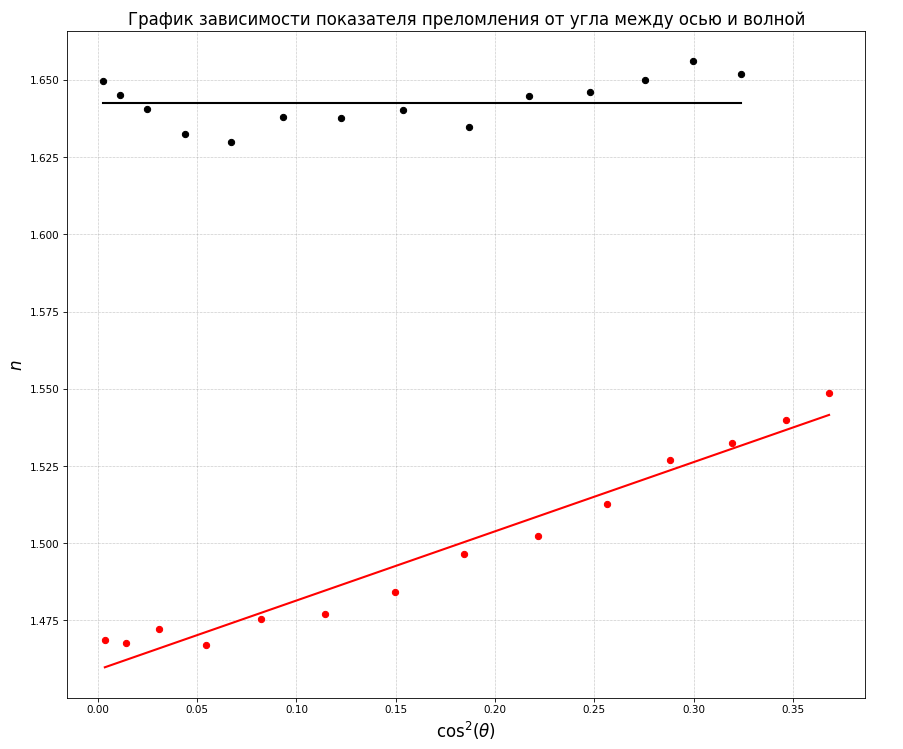
\includegraphics[width = 0.9\textwidth]{n(cos^2(theta)).png}
\end{figure}

\[n_o = (1,643 \pm 0,002), \quad \varepsilon_{n_o} = 0,12\% \]
\[n_e = (1,459 \pm 0,002), \quad \varepsilon_{n_e} = 0,13\% \]

%%%%%%%%%%%%%%%%%%%%%%%%%
\end{document}
